\begin{enumerate}[label=\thesection.\arabic*.,ref=\thesection.\theenumi]
\numberwithin{equation}{enumi}

\begin{frame}

   Q.The polar plot for the transfer function
\begin{align}
\label{ee18btech11051_eq1}
     G(s) = \frac{10(s+1)}{10+s}
\end{align} for \\0 $\leq \omega < \infty$ will be in the \\
(A) first quadrant\\
(B) second quadrant\\
(C) third quadrant\\
(D) fourth quadrant\\
\end{frame}

\begin{frame}
    The Polar plot is plotted between the magnitude and the phase angle of $G(j\omega)$ on polar coordinates by varying $\omega$ from 0 to $\infty$.
%    \begin{figure}[!h]
%    \centering
%    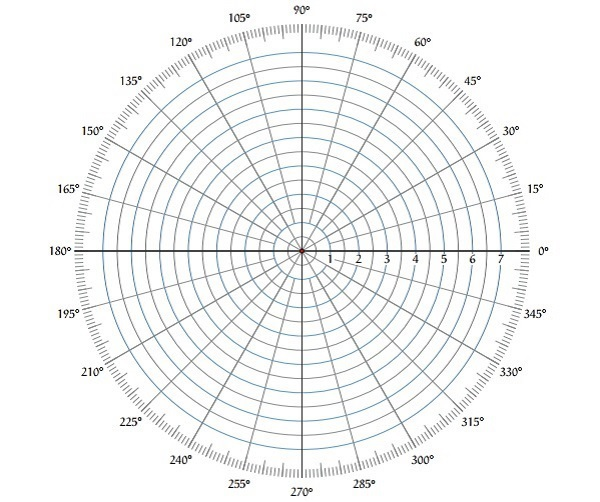
\includegraphics[width=\columnwidth]{./figs/ee18btech11051_fig1.png}
%    \caption{Polar Plot}
%    \label{fig:ee18btech11051_fig1}
%    \end{figure}
\\

  Substituting s = $j \omega$ in \eqref{ee18btech11051_eq1} gives 
\begin{align}
\label{ee18btech11051_eq2}
G(j\omega) = \frac{10(1+j\omega)}{(10+j\omega)}
\end{align}
Here, taking 1 + j$\omega$ = $\sqrt{1+{\omega}^2}e^{j\tan^{-1}(\omega)}$,
 and\\ 10 + j$\omega$ = $\sqrt{10^{2}+{\omega}^2}e^{j\tan^{-1}(\frac{\omega}{10})}$,
 \begin{align}
 \label{ee18btech11051_eq3}
G(j\omega) = 10\sqrt{\frac{1+\omega^2}{100+\omega^2}}e^{j(\tan^{-1}(\omega)-\tan^{-1}(\frac{\omega}{10}))}
\end{align}

For 0 $\leq \omega < \infty$,  0 $\leq \tan^{-1}(\omega), \tan^{-1}(\frac{\omega}{10}) < \frac{\pi}{2}$;\\
And as $\tan^{-1}$(x) is a monotonically increasing function,

[i.e.) $\frac{d}{dx}\tan^{-1}(x)$ = $\frac{1}{1+x^2} >$  0  ]\\
$\tan^{-1}(\omega) \geq \tan^{-1}(\frac{\omega}{10}) $, with equality as $\omega \rightarrow \infty$\\
So, $|G(j\omega)| > 0 $ and $0 \leq \angle G(j\omega) < \frac{\pi}{2}$
\\~\\ Therefore, the polar plot of G(s) lies in the first quadrant. \\ The plot of G(s) was plotted using the following code:
\begin{lstlisting}
    codes/ee18btech11051.py
\end{lstlisting}

\begin{center}
      \begin{figure}[!h]
      \centering
      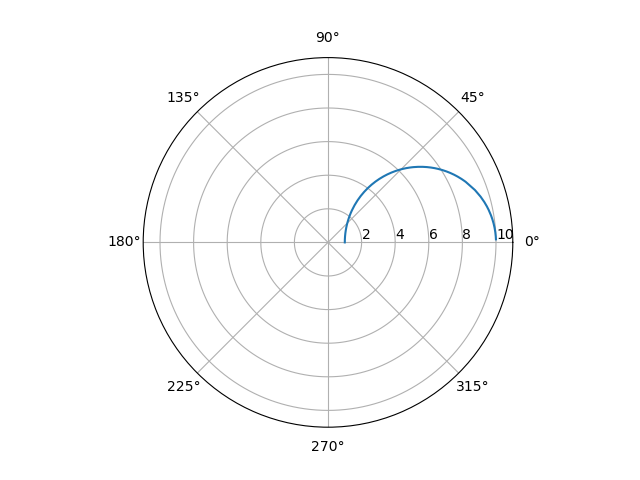
\includegraphics[width=\columnwidth]{./figs/ee18btech11051_figure1.png}
      \caption{Plot of G(s)}
      \label{fig:ee18btech11051_fig2}
      \end{figure}
\end{center}

\end{frame}

\end{enumerate}
